% Generated 2020-01-09 18:51:19 -0800
\subsection{MTConnect Device Profile} \label{model:MTConnectDeviceProfile}

\begin{figure}[ht]
  \centering
    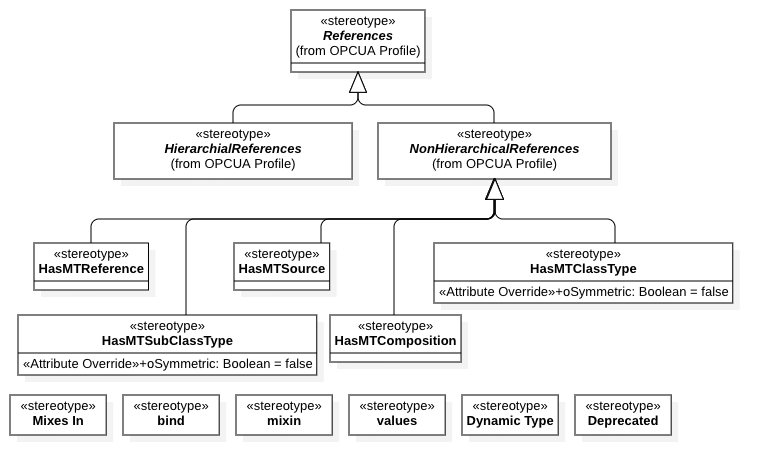
\includegraphics[width=1.0\textwidth]{./diagrams/types/MTConnectDeviceProfile.png}
  \caption{MTConnect Device Profile Diagram}
  \label{fig:MTConnectDeviceProfile}
\end{figure}

\FloatBarrier

\subsubsection{Defintion of \texttt{ <<HasMTClassType>>}}
  \label{type:HasMTClassType}

\FloatBarrier

A \gls{MTDataItem} is representated in OPC UA as a sub-type of the most appropriate \uamodel{BaseDataVariableType}. The type is derived from the MTConnect \gls{type} attribute and references the corect \mtmodel{..ClassType}


\begin{table}[ht]
\centering 
  \caption{\texttt{<<HasMTClassType>>} Definition}
  \label{table:HasMTClassType}
\fontsize{9pt}{11pt}\selectfont
\tabulinesep=3pt
\begin{tabu} to 6in {|X[-1.35]|X[-0.7]|X[-1.75]|X[-1.5]|X[-1]|X[-0.7]|} \everyrow{\hline}
\hline
\rowfont\bfseries {Attribute} & \multicolumn{5}{|l|}{Value} \\
\tabucline[1.5pt]{}
BrowseName & \multicolumn{5}{|l|}{HasMTClassType} \\
IsAbstract & \multicolumn{5}{|l|}{False} \\
Symmetric & \multicolumn{5}{|l|}{false} \\
\tabucline[1.5pt]{}
\rowfont \bfseries References & NodeClass & BrowseName & DataType & Type\-Definition & {Modeling\-Rule} \\
\multicolumn{6}{|l|}{Subtype of NonHierarchicalReferences (See \cite{UAPart5} Documentation)} \\
\end{tabu}
\end{table} 


\FloatBarrier
\subsubsection{Defintion of \texttt{ <<HasMTComposition>>}}
  \label{type:HasMTComposition}

\FloatBarrier



\begin{table}[ht]
\centering 
  \caption{\texttt{<<HasMTComposition>>} Definition}
  \label{table:HasMTComposition}
\fontsize{9pt}{11pt}\selectfont
\tabulinesep=3pt
\begin{tabu} to 6in {|X[-1.35]|X[-0.7]|X[-1.75]|X[-1.5]|X[-1]|X[-0.7]|} \everyrow{\hline}
\hline
\rowfont\bfseries {Attribute} & \multicolumn{5}{|l|}{Value} \\
\tabucline[1.5pt]{}
BrowseName & \multicolumn{5}{|l|}{HasMTComposition} \\
IsAbstract & \multicolumn{5}{|l|}{False} \\
Symmetric & \multicolumn{5}{|l|}{true} \\
\tabucline[1.5pt]{}
\rowfont \bfseries References & NodeClass & BrowseName & DataType & Type\-Definition & {Modeling\-Rule} \\
\multicolumn{6}{|l|}{Subtype of NonHierarchicalReferences (See \cite{UAPart5} Documentation)} \\
\end{tabu}
\end{table} 


\FloatBarrier
\subsubsection{Defintion of \texttt{ <<HasMTReference>>}}
  \label{type:HasMTReference}

\FloatBarrier



\begin{table}[ht]
\centering 
  \caption{\texttt{<<HasMTReference>>} Definition}
  \label{table:HasMTReference}
\fontsize{9pt}{11pt}\selectfont
\tabulinesep=3pt
\begin{tabu} to 6in {|X[-1.35]|X[-0.7]|X[-1.75]|X[-1.5]|X[-1]|X[-0.7]|} \everyrow{\hline}
\hline
\rowfont\bfseries {Attribute} & \multicolumn{5}{|l|}{Value} \\
\tabucline[1.5pt]{}
BrowseName & \multicolumn{5}{|l|}{HasMTReference} \\
IsAbstract & \multicolumn{5}{|l|}{False} \\
Symmetric & \multicolumn{5}{|l|}{true} \\
\tabucline[1.5pt]{}
\rowfont \bfseries References & NodeClass & BrowseName & DataType & Type\-Definition & {Modeling\-Rule} \\
\multicolumn{6}{|l|}{Subtype of NonHierarchicalReferences (See \cite{UAPart5} Documentation)} \\
\end{tabu}
\end{table} 


\FloatBarrier
\subsubsection{Defintion of \texttt{ <<HasMTSource>>}}
  \label{type:HasMTSource}

\FloatBarrier

The \mtmodel{Source} relation to a \gls{MTComponent} or \gls{MTDataItem}.

\begin{table}[ht]
\centering 
  \caption{\texttt{<<HasMTSource>>} Definition}
  \label{table:HasMTSource}
\fontsize{9pt}{11pt}\selectfont
\tabulinesep=3pt
\begin{tabu} to 6in {|X[-1.35]|X[-0.7]|X[-1.75]|X[-1.5]|X[-1]|X[-0.7]|} \everyrow{\hline}
\hline
\rowfont\bfseries {Attribute} & \multicolumn{5}{|l|}{Value} \\
\tabucline[1.5pt]{}
BrowseName & \multicolumn{5}{|l|}{HasMTSource} \\
IsAbstract & \multicolumn{5}{|l|}{False} \\
Symmetric & \multicolumn{5}{|l|}{true} \\
\tabucline[1.5pt]{}
\rowfont \bfseries References & NodeClass & BrowseName & DataType & Type\-Definition & {Modeling\-Rule} \\
\multicolumn{6}{|l|}{Subtype of NonHierarchicalReferences (See \cite{UAPart5} Documentation)} \\
\end{tabu}
\end{table} 


\FloatBarrier
\subsubsection{Defintion of \texttt{ <<HasMTSubClassType>>}}
  \label{type:HasMTSubClassType}

\FloatBarrier

A \gls{MTDataItem} is representated in OPC UA as a sub-type of the most appropriate \uamodel{BaseDataVariableType}. 
The sub-type is derived from the MTConnect \gls{subType} attribute and references the corect \mtmodel{..ClassType}.

\begin{table}[ht]
\centering 
  \caption{\texttt{<<HasMTSubClassType>>} Definition}
  \label{table:HasMTSubClassType}
\fontsize{9pt}{11pt}\selectfont
\tabulinesep=3pt
\begin{tabu} to 6in {|X[-1.35]|X[-0.7]|X[-1.75]|X[-1.5]|X[-1]|X[-0.7]|} \everyrow{\hline}
\hline
\rowfont\bfseries {Attribute} & \multicolumn{5}{|l|}{Value} \\
\tabucline[1.5pt]{}
BrowseName & \multicolumn{5}{|l|}{HasMTSubClassType} \\
IsAbstract & \multicolumn{5}{|l|}{False} \\
Symmetric & \multicolumn{5}{|l|}{false} \\
\tabucline[1.5pt]{}
\rowfont \bfseries References & NodeClass & BrowseName & DataType & Type\-Definition & {Modeling\-Rule} \\
\multicolumn{6}{|l|}{Subtype of NonHierarchicalReferences (See \cite{UAPart5} Documentation)} \\
\end{tabu}
\end{table} 


\FloatBarrier
\subsubsection{Defintion of \texttt{ <<Mixes In>>}}
  \label{type:Mixes In}

\FloatBarrier



\FloatBarrier
\subsubsection{Defintion of \texttt{ <<mixin>>}}
  \label{type:mixin}

\FloatBarrier

The mixin pattern injects the properties and operations into the types
that are related to the using the \texttt{Mixes In} dependency. Mixins allow for
lightweight multiple inheritance. Since OPC/UA does not allow for multiple inheritance
and the MTConnect  types require the same set of properties when they are sub-typed
from existing OPC/UA types, this mechanism allows for this relationship to be expressed.


\FloatBarrier
\subsubsection{Defintion of \texttt{ <<values>>}}
  \label{type:values}

\FloatBarrier

For controlled vocabularies of enumerated types, specifies the relationship to the allowable
values for the type


\FloatBarrier
